\documentclass{article}
\usepackage{tikz}
\usepackage{amsmath}
\usetikzlibrary{angles,quotes}
\usetikzlibrary{decorations.pathmorphing,calc}
\begin{document}
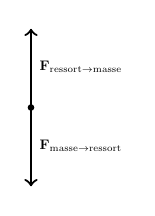
\begin{tikzpicture}[scale=1]
% Paramètres
\def\x{0}
\def\dx{0.5}
\def\w{0.3}
\def\h{0.5}
\def\F{1}
\def\y{-2}
\def\dy{0}
% Point d’application de la force
\coordinate (P) at (\x+\dx+0.3*\w,\y+\dy-0.5*\h);
\draw[thick, ->] (\x+\dx+0.3*\w,\y+\dy-0.5*\h)
 -- ++(0,\F)
 node[midway,right=18,above=-3.5,scale=0.5]
 {$\mathbf{F_{\text{ressort}\rightarrow\text{masse}}}$};
\draw[thick, ->] (\x+\dx+0.3*\w,\y+\dy-0.5*\h)
 -- ++(0,-\F)
 node[midway,right=18,above=-3.5,scale=0.5]
 {$\mathbf{F_{\text{masse}\rightarrow\text{ressort}}}$};
% Point matérialisant le point d’application
\fill (P) circle (1.2pt);
\end{tikzpicture}
\end{document}